
\vspace{0.15cm}
\begin{flushleft}
	{\color{blue!50!green}\fbox{\fontfamily{qag}\bfseries\selectfont PHẦN I. Câu trắc nghiệm nhiều phương án lựa chọn (3,0 điểm)}}
	\textit{\small (Thí sinh trả lời từ câu 1 đến câu 12. Mỗi câu hỏi thí sinh chỉ chọn một phương án.)}
\end{flushleft}
\setcounter{ex}{0}
\setcounter{bt}{0}

% Câu 1
\begin{ex}
	Mỗi ngày bố của bạn An chở bạn ấy từ nhà đến trường mất $20\text{ phút}$. Hôm nay là ngày thi nên bố bạn ấy chạy xe nhanh hơn và đến trường sớm hơn thường ngày $5\text{ phút}$. Biết quãng đường từ nhà bạn An đến trường là $10\text{ km}$. Tốc độ trung bình của xe hôm nay là
	\choice
	{\True $40\text{ km/h}$}
	{$50\text{ km/h}$}
	{$30\text{ km/h}$}
	{$60\text{ km/h}$}
	\loigiai{
		Thời gian chuyển động hôm nay: $t' = 20 - 5 = 15\text{ phút} = 0{,}25\text{ h}$.\par
		Tốc độ trung bình của xe hôm nay:\par
		\[v_{\text{tb}} = \frac{s}{t'} = \frac{10}{0{,}25} = 40\text{ km/h}.\]
	}
\end{ex}

% Câu 2
\begin{ex}
	Hình dưới mô tả đồ thị độ dịch chuyển -- thời gian của hai xe chuyển động thẳng trong cùng một khoảng thời gian. Chọn câu đúng.
	\begin{center}
		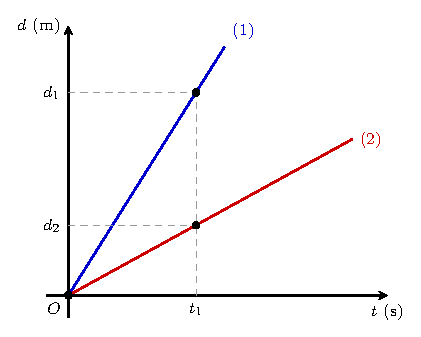
\includegraphics[width=4.8cm]{fig_cau2.pdf}
	\end{center}
	\choice
	{\True Tốc độ vật 1 lớn hơn tốc độ vật 2}
	{Vận tốc vật 1 nhỏ hơn vận tốc vật 2}
	{Tốc độ vật 2 lớn hơn tốc độ vật 1}
	{Vận tốc vật 1 có thể lớn hơn, nhỏ hơn hoặc bằng vận tốc vật 2}
	\loigiai{
		Trong đồ thị $d - t$ của chuyển động thẳng đều, độ dốc của đường biểu diễn cho biết vận tốc: $v = \dfrac{\Delta d}{\Delta t}$.\par
		Đường (1) dốc hơn đường (2): trong cùng thời gian $t_1$ thì $d_1 > d_2$, suy ra $v_1 > v_2$. Vậy tốc độ vật 1 lớn hơn tốc độ vật 2.\par
	}
\end{ex}

% Câu 3
\begin{ex}
	Hãy sắp xếp các phương pháp nghiên cứu vật lí sau theo đúng tiến trình lịch sử phát triển của vật lí học:\\ (1) Sử dụng phương pháp thực nghiệm để tìm hiểu thế giới tự nhiên.\\ (2) Dựa trên quan sát và suy luận chủ quan để tìm hiểu thế giới tự nhiên.\\ (3) Sử dụng kết hợp các mô hình lí thuyết tìm hiểu thế giới vi mô và thí nghiệm để kiểm chứng.
	\choice
	{(1) -- (2) -- (3)}
	{\True (2) -- (1) -- (3)}
	{(2) -- (3) -- (1)}
	{(1) -- (3) -- (2)}
	\loigiai{
		Tiến trình phát triển của vật lí học gồm ba giai đoạn:\par
		-- Tiền vật lí: tìm hiểu tự nhiên dựa trên quan sát và suy luận chủ quan (2).\par
		-- Vật lí cổ điển: phương pháp thực nghiệm do Galilei khởi xướng (1).\par
		-- Vật lí hiện đại: kết hợp mô hình lí thuyết về thế giới vi mô với thí nghiệm kiểm chứng (3).\par
		Thứ tự đúng: (2) -- (1) -- (3).\par
	}
\end{ex}

% Câu 4
\begin{ex}
	Hai vật có khối lượng $m_1 < m_2$ được thả rơi tự do tại cùng một độ cao trong chân không, vận tốc tương ứng khi chạm đất là $v_1$ và $v_2$. Kết luận nào sau đây đúng?
	\choice
	{$v_1 \ge v_2$ hoặc $v_1 < v_2$}
	{\True $v_1 = v_2$}
	{$v_1 > v_2$}
	{$v_1 < v_2$}
	\loigiai{
		Vận tốc chạm đất của vật rơi tự do $v = \sqrt{2gh}$ không phụ thuộc khối lượng, chỉ phụ thuộc độ cao $h$. Hai vật rơi từ cùng độ cao nên $v_1 = v_2$.\par
	}
\end{ex}

% Câu 5
\begin{ex}
	Hai vật được thả rơi tự do đồng thời từ hai độ cao khác nhau $h_1$ và $h_2$. Thời gian rơi của vật thứ nhất lớn gấp ba lần thời gian rơi của vật thứ hai. Bỏ qua lực cản của không khí. Tỉ số các độ cao tương ứng là
	\choice
	{\True $\dfrac{h_1}{h_2} = 9$}
	{$\dfrac{h_1}{h_2} = 3$}
	{$\dfrac{h_1}{h_2} = \dfrac{1}{9}$}
	{$\dfrac{h_1}{h_2} = \dfrac{1}{3}$}
	\loigiai{
		Độ cao rơi tự do: $h = \dfrac{1}{2}gt^2$, suy ra\par
		\[\frac{h_1}{h_2} = \left(\frac{t_1}{t_2}\right)^2 = 3^2 = 9.\]
	}
\end{ex}

% Câu 6
\begin{ex}
	Trong các trường hợp dưới đây, trị số vận tốc nào là tốc độ trung bình?
	\choice
	{\True Xe lửa chạy với tốc độ $40\text{ km/h}$ trên hành trình từ Huế ra Quảng Trị}
	{Tốc độ của bạn Long đo được lúc đúng 7 giờ 15 phút là $5\text{ km/h}$}
	{Viên đạn bay ra khỏi nòng súng với tốc độ $600\text{ m/s}$}
	{Tốc độ của đầu búa máy ngay tại thời điểm va chạm là $8\text{ m/s}$}
	\loigiai{
		Tốc độ trung bình đặc trưng cho độ nhanh chậm trên cả một quãng đường (hành trình Huế -- Quảng Trị).\par
		Các trị số đo tại một thời điểm hay một vị trí xác định (lúc 7 giờ 15 phút, khi ra khỏi nòng súng, lúc va chạm) là tốc độ tức thời.\par
	}
\end{ex}

% Câu 7
\begin{ex}
	Gia tốc rơi tự do được xác định qua phép đo độ cao $h$ và thời gian rơi $t$ theo công thức $g = \dfrac{2h}{t^2}$. Biểu thức xác định sai số tuyệt đối $\Delta g$ của phép đo là
	\choice
	{$\Delta g = \overline{g}\left(2\dfrac{\Delta h}{\overline{h}} + \dfrac{\Delta t}{\overline{t}}\right)$}
	{$\Delta g = \overline{g}\left(\dfrac{\Delta h}{\overline{h}} + \dfrac{\Delta t}{\overline{t}}\right)$}
	{\True $\Delta g = \overline{g}\left(\dfrac{\Delta h}{\overline{h}} + 2\dfrac{\Delta t}{\overline{t}}\right)$}
	{$\Delta g = \dfrac{\Delta h}{\Delta t^2}$}
	\loigiai{
		Với $g = 2h\,t^{-2}$, sai số tỉ đối bằng tổng sai số tỉ đối của các thừa số (nhân với số mũ tương ứng):\par
		\[\frac{\Delta g}{\overline{g}} = \frac{\Delta h}{\overline{h}} + 2\frac{\Delta t}{\overline{t}} \Rightarrow \Delta g = \overline{g}\left(\frac{\Delta h}{\overline{h}} + 2\frac{\Delta t}{\overline{t}}\right).\]
	}
\end{ex}

% Câu 8
\begin{ex}
	Một vật chuyển động thẳng nhanh dần đều không vận tốc đầu với phương trình độ dịch chuyển $d = 3t^2\text{ (m)}$. Gọi $v$ là vận tốc của vật tại thời điểm $t$, $S$ là quãng đường vật đi được sau thời gian $t$. Hệ thức đúng là
	\choice
	{\True $v^2 = 12S$}
	{$v^2 = 6S$}
	{$v^2 = 4S$}
	{$v^2 = 8S$}
	\loigiai{
		So sánh $d = v_0t + \dfrac{1}{2}at^2 = 3t^2$ ta được $v_0 = 0$ và $a = 6\text{ m/s}^2$.\par
		Vật chuyển động thẳng không đổi chiều nên $S = d$. Áp dụng hệ thức độc lập thời gian:\par
		\[v^2 - v_0^2 = 2aS \Rightarrow v^2 = 2 \cdot 6 \cdot S = 12S.\]
	}
\end{ex}

% Câu 9
\begin{ex}
	Một vật chuyển động thẳng biến đổi đều dọc theo trục $Ox$. Tại thời điểm $t_0$ vận tốc của vật là $v_0$, tại thời điểm $t$ vận tốc của vật là $v$. Gia tốc của vật được xác định bằng công thức
	\choice
	{$a = \dfrac{v^2 + v_0^2}{t - t_0}$}
	{\True $a = \dfrac{v - v_0}{t - t_0}$}
	{$a = \dfrac{v^2 - v_0^2}{t - t_0}$}
	{$a = \dfrac{v + v_0}{t + t_0}$}
	\loigiai{
		Gia tốc là độ biến thiên vận tốc trong một đơn vị thời gian: $a = \dfrac{\Delta v}{\Delta t} = \dfrac{v - v_0}{t - t_0}$.\par
	}
\end{ex}

% Câu 10
\begin{ex}
	Khi lắp ráp và sử dụng các thiết bị điện trong phòng thực hành Vật lí, thao tác nào sau đây là yêu cầu bắt buộc và quan trọng nhất?
	\choice
	{Không cần quan tâm sử dụng đúng chức năng của thiết bị}
	{Chỉ cần quan sát sơ bộ hình dáng bên ngoài rồi bật công tắc ngay}
	{\True Quan sát kĩ các kí hiệu cảnh báo và thông số kĩ thuật trên thiết bị để sử dụng đúng chức năng, đúng điện áp}
	{Bật nguồn điện trước rồi mới cắm dây tiến hành thí nghiệm}
	\loigiai{
		Để đảm bảo an toàn cho người và thiết bị, trước khi sử dụng phải quan sát kĩ các kí hiệu cảnh báo, nhãn thông số kĩ thuật để dùng đúng chức năng và đúng điện áp.\par
	}
\end{ex}

% Câu 11
\begin{ex}
	Cho các phép đo: (1) dùng thước đo chiều cao; (2) dùng đồng hồ bấm giây đo thời gian; (3) đo gia tốc rơi tự do thông qua công thức; (4) đo tốc độ chuyển động thông qua quãng đường và thời gian. Các phép đo gián tiếp là
	\choice
	{(1), (2), (4)}
	{(1), (2)}
	{(2), (3), (4)}
	{\True (3), (4)}
	\loigiai{
		Phép đo trực tiếp: đọc kết quả ngay trên dụng cụ đo -- (1), (2).\par
		Phép đo gián tiếp: xác định qua công thức liên hệ với các đại lượng đo trực tiếp -- (3) $g = \dfrac{2h}{t^2}$ và (4) $v = \dfrac{s}{t}$.\par
	}
\end{ex}

% Câu 12
\begin{ex}
	Đồ thị vận tốc -- thời gian $(v - t)$ của một vật chuyển động thẳng dọc theo trục $Ox$ đi qua ba điểm $A$, $B$, $C$ như hình vẽ. Quãng đường vật đi được trong khoảng thời gian từ $0\text{ s}$ đến $5\text{ s}$ bằng
	\begin{center}
		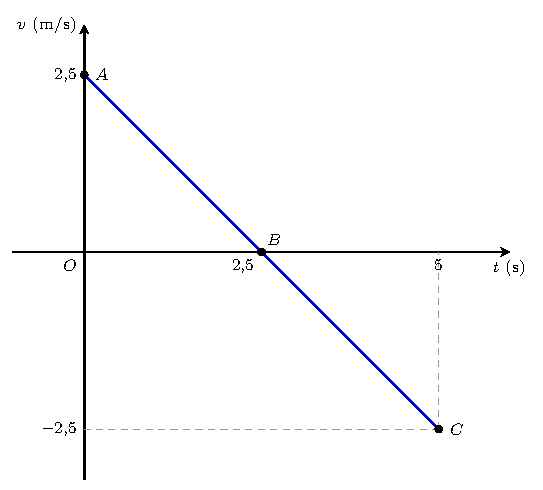
\includegraphics[width=5.2cm]{fig_cau12.pdf}
	\end{center}
	\choice
	{\True $6{,}25\text{ m}$}
	{$7{,}25\text{ m}$}
	{$6\text{ m}$}
	{$12{,}5\text{ m}$}
	\loigiai{
		Quãng đường bằng tổng diện tích các phần giới hạn bởi đồ thị $v - t$ và trục $Ot$ (lấy giá trị dương):\par
		-- Từ $0$ đến $2{,}5\text{ s}$ (tam giác $OAB$): $s_1 = \dfrac{1}{2} \cdot 2{,}5 \cdot 2{,}5 = 3{,}125\text{ m}$.\par
		-- Từ $2{,}5\text{ s}$ đến $5\text{ s}$ (vật đổi chiều, tam giác dưới trục): $s_2 = \dfrac{1}{2} \cdot 2{,}5 \cdot 2{,}5 = 3{,}125\text{ m}$.\par
		\[s = s_1 + s_2 = 3{,}125 + 3{,}125 = 6{,}25\text{ m}.\]
	}
\end{ex}

\vspace{0.15cm}
\begin{flushleft}
	{\color{blue!50!green}\fbox{\fontfamily{qag}\bfseries\selectfont PHẦN II. Câu trắc nghiệm đúng sai (2,0 điểm)}}
	\textit{\small (Thí sinh trả lời từ câu 1 đến câu 2. Trong mỗi ý a), b), c), d) ở mỗi câu, thí sinh chọn đúng hoặc sai.)}
\end{flushleft}
\setcounter{ex}{0}
\setcounter{bt}{0}

% Phần II Câu 1
\begin{ex}
	Một quả cầu bắt đầu lăn không vận tốc đầu từ đỉnh $A$ của một dốc thẳng dài $100\text{ m}$, sau $10\text{ s}$ thì tới chân dốc $B$. Từ $B$, quả cầu tiếp tục lăn chậm dần đều trên mặt phẳng ngang thêm $50\text{ m}$ thì dừng lại tại $C$. Chọn chiều dương là chiều chuyển động của quả cầu.
	\begin{center}
		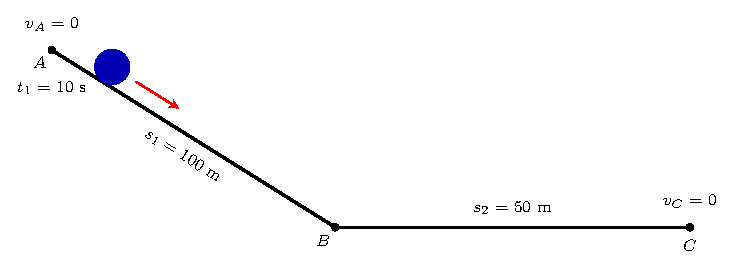
\includegraphics[width=10.5cm]{fig_cau13.pdf}
	\end{center}
	\choiceTF[t]
	{Gia tốc của quả cầu khi lăn xuống dốc $AB$ bằng $2{,}5\text{ m/s}^2$.}
	{\True Vận tốc của quả cầu tại chân dốc $B$ bằng $20\text{ m/s}$.}
	{\True Độ lớn gia tốc của quả cầu khi lăn chậm dần đều trên đoạn $BC$ bằng $4\text{ m/s}^2$.}
	{\True Tổng thời gian chuyển động của quả cầu từ $A$ đến khi dừng lại tại $C$ bằng $15\text{ s}$.}
	\loigiai{
		{\color{red!80!black}\textbf{a) Sai.}} Trên dốc $AB$: $s_1 = \dfrac{1}{2}a_1t_1^2 \Rightarrow 100 = \dfrac{1}{2}a_1 \cdot 10^2 \Rightarrow a_1 = 2\text{ m/s}^2 \ne 2{,}5\text{ m/s}^2$.\par
		{\color{green!50!black}\textbf{b) Đúng.}} $v_B = a_1t_1 = 2 \cdot 10 = 20\text{ m/s}$.\par
		{\color{green!50!black}\textbf{c) Đúng.}} Trên $BC$: $v_C^2 - v_B^2 = 2a_2s_2 \Rightarrow 0 - 20^2 = 2a_2 \cdot 50 \Rightarrow a_2 = -4\text{ m/s}^2$, độ lớn $4\text{ m/s}^2$.\par
		{\color{green!50!black}\textbf{d) Đúng.}} Thời gian trên $BC$: $t_2 = \dfrac{v_C - v_B}{a_2} = \dfrac{0 - 20}{-4} = 5\text{ s}$. Tổng thời gian: $t = t_1 + t_2 = 10 + 5 = 15\text{ s}$.\par
	}
\end{ex}

% Phần II Câu 2
\begin{ex}
	Một nhóm học sinh làm thí nghiệm đo tốc độ trung bình của một xe chuyển động thẳng từ $A$ đến $B$. Dùng thước đo được quãng đường $s = 0{,}500 \pm 0{,}002\text{ (m)}$. Dùng đồng hồ hiện số có sai số dụng cụ $0{,}001\text{ s}$ đo thời gian chuyển động, kết quả 4 lần đo ghi ở bảng sau:

\begin{center}\begin{tabular}{|c|c|c|c|c|}\hline \textbf{Lần đo} & \textbf{1} & \textbf{2} & \textbf{3} & \textbf{4} \\ \hline \textbf{$t$ (s)} & 0,776 & 0,778 & 0,772 & 0,774 \\ \hline\end{tabular}\end{center}
	\choiceTF[t]
	{Phép đo tốc độ trung bình trong thí nghiệm này là phép đo trực tiếp.}
	{\True Kết quả đo thời gian là $t = 0{,}775 \pm 0{,}003\text{ (s)}$.}
	{\True Kết quả đo tốc độ trung bình là $v = 0{,}645 \pm 0{,}005\text{ (m/s)}$.}
	{Sai số tỉ đối của phép đo tốc độ trung bình là $\delta v = 0{,}5\%$.}
	\loigiai{
		{\color{red!80!black}\textbf{a) Sai.}} Tốc độ trung bình được tính qua công thức $v = \dfrac{s}{t}$ từ hai đại lượng đo trực tiếp nên là phép đo gián tiếp.\par
		{\color{green!50!black}\textbf{b) Đúng.}} $\overline{t} = \dfrac{0{,}776 + 0{,}778 + 0{,}772 + 0{,}774}{4} = 0{,}775\text{ s}$; $\overline{\Delta t} = \dfrac{0{,}001 + 0{,}003 + 0{,}003 + 0{,}001}{4} = 0{,}002\text{ s}$. Vậy $\Delta t = 0{,}002 + 0{,}001 = 0{,}003\text{ s}$ và $t = 0{,}775 \pm 0{,}003\text{ s}$.\par
		{\color{green!50!black}\textbf{c) Đúng.}} $\overline{v} = \dfrac{0{,}500}{0{,}775} \approx 0{,}645\text{ m/s}$; $\delta v = \dfrac{0{,}002}{0{,}500} + \dfrac{0{,}003}{0{,}775} \approx 0{,}0079$; $\Delta v = \overline{v}\cdot\delta v \approx 0{,}005\text{ m/s}$. Vậy $v = 0{,}645 \pm 0{,}005\text{ m/s}$.\par
		{\color{red!80!black}\textbf{d) Sai.}} $\delta v \approx 0{,}79\% \approx 0{,}8\% \ne 0{,}5\%$.\par
	}
\end{ex}

\vspace{0.15cm}
\begin{flushleft}
	{\color{blue!50!green}\fbox{\fontfamily{qag}\bfseries\selectfont PHẦN III. Câu trắc nghiệm trả lời ngắn (2,0 điểm)}}
	\textit{\small (Thí sinh trả lời từ câu 1 đến câu 4.)}
\end{flushleft}
\setcounter{ex}{0}
\setcounter{bt}{0}

% Phần III Câu 1
\begin{ex}
	Bạn Khánh Linh chạy bộ trên một đường thẳng trong $10\text{ phút}$. Trong $4\text{ phút}$ đầu, bạn chạy đều với tốc độ $4\text{ m/s}$; thời gian còn lại bạn chạy đều với tốc độ $3\text{ m/s}$. Tốc độ trung bình của bạn Khánh Linh trong $10\text{ phút}$ đó là bao nhiêu $\text{m/s}$?
	\par\shortans[oly]{3,4}
	\loigiai{
		$t_1 = 4\text{ phút} = 240\text{ s}$; $t_2 = 6\text{ phút} = 360\text{ s}$; tổng thời gian $t = 600\text{ s}$.\par
		Quãng đường: $s = v_1t_1 + v_2t_2 = 4 \cdot 240 + 3 \cdot 360 = 2040\text{ m}$.\par
		\[v_{\text{tb}} = \frac{s}{t} = \frac{2040}{600} = 3{,}4\text{ m/s}.\]
	}
\end{ex}

% Phần III Câu 2
\begin{ex}
	Trong đợt lũ lụt tại các tỉnh miền Bắc đầu tháng 10 năm 2025, dòng nước lũ chảy với tốc độ khoảng $4\text{ m/s}$ so với bờ. Một ca nô cứu hộ chạy ngược dòng với tốc độ $8\text{ m/s}$ so với dòng nước để tiếp cận một mái nhà có người mắc kẹt cách trạm xuất phát $1920\text{ m}$. Thời gian để ca nô tiếp cận chỗ người bị nạn là bao nhiêu phút?
	\par\shortans[oly]{8}
	\loigiai{
		Vận tốc ca nô so với bờ khi chạy ngược dòng: $v = v_{\text{cn/n}} - v_{\text{n/b}} = 8 - 4 = 4\text{ m/s}$.\par
		\[t = \frac{s}{v} = \frac{1920}{4} = 480\text{ s} = 8\text{ phút}.\]
	}
\end{ex}

% Phần III Câu 3
\begin{ex}
	Hình vẽ là đồ thị độ dịch chuyển -- thời gian $(d - t)$ của một vật chuyển động thẳng. Quãng đường vật đi được từ thời điểm $t = 0$ đến thời điểm $t = 4\text{ s}$ là bao nhiêu mét?
	\begin{center}
		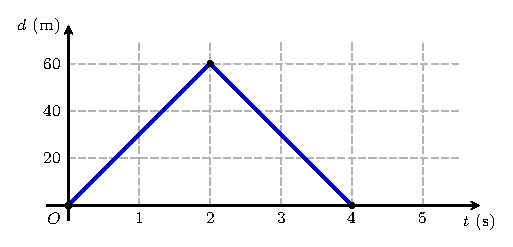
\includegraphics[width=6.8cm]{fig_cau17.pdf}
	\end{center}
	\par\shortans[oly]{120}
	\loigiai{
		-- Từ $0$ đến $2\text{ s}$: độ dịch chuyển tăng từ $0$ lên $60\text{ m}$, vật đi theo chiều dương được $s_1 = 60\text{ m}$.\par
		-- Từ $2\text{ s}$ đến $4\text{ s}$: độ dịch chuyển giảm từ $60\text{ m}$ về $0$, vật đổi chiều và đi được $s_2 = 60\text{ m}$.\par
		\[s = s_1 + s_2 = 60 + 60 = 120\text{ m}.\]
	}
\end{ex}

% Phần III Câu 4
\begin{ex}
	Hai giọt nước mưa rơi tự do từ cùng một độ cao $h$, giọt thứ hai rơi sau giọt thứ nhất $1\text{ s}$. Khi giọt thứ nhất vừa chạm đất thì giọt thứ hai còn cách mặt đất $45\text{ m}$. Bỏ qua lực cản không khí, lấy $g = 10\text{ m/s}^2$. Độ cao $h$ bằng bao nhiêu mét?
	\par\shortans[oly]{125}
	\loigiai{
		Gọi $t$ là thời gian rơi của giọt thứ nhất: $h = \dfrac{1}{2}gt^2 = 5t^2$.\par
		Khi đó giọt thứ hai đã rơi $(t - 1)$ giây: $s_2 = 5(t - 1)^2$.\par
		\[h - s_2 = 45 \Rightarrow 5t^2 - 5(t - 1)^2 = 45 \Rightarrow 5(2t - 1) = 45 \Rightarrow t = 5\text{ s}.\]
		\[h = 5 \cdot 5^2 = 125\text{ m}.\]
	}
\end{ex}

\vspace{0.15cm}
\begin{flushleft}
	{\color{blue!50!green}\fbox{\fontfamily{qag}\bfseries\selectfont PHẦN IV. Tự luận (3,0 điểm)}}
	\textit{\small (Thí sinh trình bày lời giải từ câu 1 đến câu 3.)}
\end{flushleft}
\setcounter{ex}{0}
\setcounter{bt}{0}

% Phần IV Câu 1
\begin{ex}
	Một ô tô chuyển động thẳng đều với tốc độ $80\text{ km/h}$ từ $A$ về hướng Đông. Sau khi đi được $32\text{ km}$, ô tô rẽ trái chuyển động thẳng đều về hướng Bắc với tốc độ $40\text{ km/h}$ trong $36\text{ phút}$ thì đến $B$. Tính:
	\par \textbf{a)} Quãng đường ô tô đi từ $A$ đến $B$. \par \textbf{b)} Thời gian ô tô đi từ $A$ đến $B$. \par \textbf{c)} Tốc độ trung bình và độ lớn vận tốc trung bình của ô tô trên cả hành trình.
	\loigiai{
		\textbf{a)} $t_2 = 36\text{ phút} = 0{,}6\text{ h}$, $s_2 = v_2t_2 = 40 \cdot 0{,}6 = 24\text{ km}$. Quãng đường: $s = s_1 + s_2 = 32 + 24 = 56\text{ km}$.\par
		\textbf{b)} $t_1 = \dfrac{s_1}{v_1} = \dfrac{32}{80} = 0{,}4\text{ h}$. Thời gian: $t = t_1 + t_2 = 0{,}4 + 0{,}6 = 1\text{ h}$.\par
		\textbf{c)} Tốc độ trung bình: $v_{\text{tb}} = \dfrac{s}{t} = \dfrac{56}{1} = 56\text{ km/h}$.\par
		Hai chặng vuông góc nên độ dịch chuyển: $d = \sqrt{s_1^2 + s_2^2} = \sqrt{32^2 + 24^2} = 40\text{ km}$.\par
		Độ lớn vận tốc trung bình: $v = \dfrac{d}{t} = \dfrac{40}{1} = 40\text{ km/h}$.\par
	}
\end{ex}

% Phần IV Câu 2
\begin{ex}
	Một ô tô đang chạy thẳng đều với tốc độ $72\text{ km/h}$ thì hãm phanh, chuyển động thẳng chậm dần đều và đi thêm $250\text{ m}$ nữa thì dừng hẳn. Chọn chiều dương là chiều chuyển động. Tính:
	\par \textbf{a)} Gia tốc $a$ của ô tô. \par \textbf{b)} Quãng đường ô tô đi được trong $10\text{ s}$ cuối cùng trước khi dừng hẳn.
	\loigiai{
		\textbf{a)} $v_0 = 72\text{ km/h} = 20\text{ m/s}$, $v = 0$. Áp dụng $v^2 - v_0^2 = 2as$:\par
		\[0 - 20^2 = 2 \cdot a \cdot 250 \Rightarrow a = -0{,}8\text{ m/s}^2.\]
		\textbf{b)} Thời gian hãm phanh: $t = \dfrac{0 - 20}{-0{,}8} = 25\text{ s} > 10\text{ s}$.\par
		Xét ngược thời gian, $10\text{ s}$ cuối của chuyển động chậm dần đều tương đương $10\text{ s}$ đầu của chuyển động nhanh dần đều không vận tốc đầu với gia tốc $0{,}8\text{ m/s}^2$:\par
		\[s' = \frac{1}{2}|a|t'^2 = \frac{1}{2} \cdot 0{,}8 \cdot 10^2 = 40\text{ m}.\]
	}
\end{ex}

% Phần IV Câu 3
\begin{ex}
	Hai xe xuất phát cùng lúc từ trạng thái nghỉ, chuyển động thẳng nhanh dần đều cùng chiều dương. Hình vẽ là đồ thị quãng đường -- thời gian $(s - t)$ của xe (1) và xe (2). Dựa vào đồ thị, hãy tính giá trị $S_1$.
	\begin{center}
		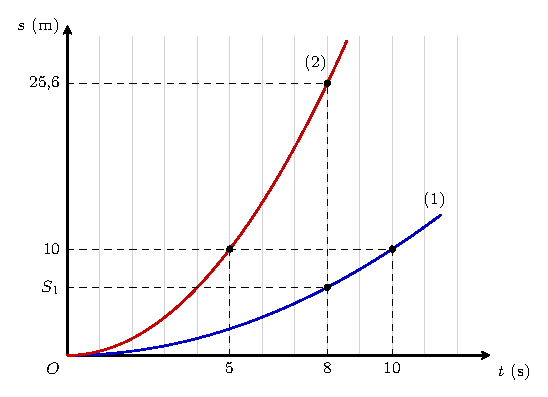
\includegraphics[width=7.0cm]{fig_cau21.pdf}
	\end{center}
	\loigiai{
		Với chuyển động nhanh dần đều không vận tốc đầu: $s = \dfrac{1}{2}at^2$.\par
		-- Xe (2) đi được $10\text{ m}$ sau $5\text{ s}$: $a_2 = \dfrac{2 \cdot 10}{5^2} = 0{,}8\text{ m/s}^2$ (kiểm tra: tại $t = 8\text{ s}$, $s_2 = \dfrac{1}{2} \cdot 0{,}8 \cdot 8^2 = 25{,}6\text{ m}$, đúng như đồ thị).\par
		-- Xe (1) đi được $10\text{ m}$ sau $10\text{ s}$: $a_1 = \dfrac{2 \cdot 10}{10^2} = 0{,}2\text{ m/s}^2$.\par
		Tại $t = 8\text{ s}$, quãng đường xe (1) đi được:\par
		\[S_1 = \frac{1}{2}a_1t^2 = \frac{1}{2} \cdot 0{,}2 \cdot 8^2 = 6{,}4\text{ m}.\]
	}
\end{ex}
